\documentclass{TDP003mall}
\usepackage{graphicx}
\graphicspath{ {bilder/} }


\newcommand{\version}{Version 1.0}
\author{Gustav P Svensson, \url{gussv375@student.liu.se}\\
  Love Bäckman, \url{lovba497@student.liu.se}}
\title{X Runner}
\date{2016-xx-xx}
\rhead{Gustav P Svensson\\
Love Backman}



\begin{document}
\projectpage

\tableofcontents
\newpage

\section{Revisionshistorik}
\begin{table}[!h]
\begin{tabularx}{\linewidth}{|l|X|l|}
\hline
Ver. & Revisionsbeskrivning & Datum \\\hline
0.1 & Ett första utkast & 16110 \\\hline
\end{tabularx}
\end{table}


\section{Spelide}
X Runner är ett plattformsracingspel som utspelar sig i en 2D-värld med en kamera som följer spelarens karaktär från sidan. Spelarens uppgift är att klara av en bana så fort som möjligt, vilket denne gör genom att ta sig från punkt A till punkt B samtidigt som hänsyn måste tas till diverse ickespelarkaraktärer (NPC's) och specialblock som påverkar spelarens hastighet. Till en början kommer tävlingsmomentet utgöras av att försöka slå det nuvarande rekordet, men i mån av tid kommer även online multiplayer att implementeras.

\section{Målgrupp}
Spelets målgrupp är personer i alla åldrar som gillar utmanande plattformsracingspel likt Pixelvania.

\section{Spelupplevelse}
Det som gör spelet underhållande är utmaningen och strävan att alltid bli bättre för att så småningom, till en början lite då och då, och därefter konsekvent, kunna få till ``perfect runs''. Om det därtill finns flera banor slutar inte utmaningen där, utan då blir utmaningen att konsekvent hålla en hög nivå på olika banor.

\newpage

\section{Spelmekanik}
\subsection{In-game}
\subsubsection{Spelare}
Spelaren kan röra sig i sidled samt hoppa. Spelaren påverkas även av gravitationen och faller således mot marken om denne inte befinner sig på ett solidt block.
\\\\
I mån av tid kommer spelaren även att kunna walljumpa samt öka sin hastighet genom att hoppa med sidledsrörelse flera på varandra efterföljande gånger.
\subsubsection{Kontroller}
\begin{tabular}{|c|c|}
\hline
\textbf{Knapptryck} & \textbf{Händelse} \\\hline
W eller $\uparrow$ & Spelaren hoppar \\\hline
A eller $\leftarrow$ & Spelaren går åt vänster \\\hline
D eller $\rightarrow$ & Spelaren går åt höger \\\hline
ESC & Gå till startmenyn \\\hline
\end{tabular}

\subsubsection{NPC's \& Specialblock}
NPC's kommer röra sig enligt en förbestämd algoritm. Följande NPC's och specialblock kommer finnas i spelet och detta är deras effekter:
\\\\
\begin{tabular}{|l|l|l|}
\hline
\textbf{NPC / Specialblock} & \textbf{Effekt vid kollision med spelare} & \textbf{Övriga effekter}\\\hline
Slow Bird & Spelarens hastighet minskar i ett antal sekunder & \\\hline
Boost Bird & Spelarens hastighet ökar i ett antal sekunder & Spawnar Net from Boost Bird\\\hline
Net from Boost Bird & Spelaren kan inte röra sig i ett antal sekunder + despawn & \\\hline
Quicksand & Spelarens hastighet minskar och spelaren kan inte hoppa & \\\hline
Goalblock & Banan är avklarad & \\\hline
\end{tabular}

\subsubsection{Kamera}
Kameran kommer förflytta sig så att spelaren alltid är centrerad på skärmen.

\subsection{Startmeny}
I startmenyn kan spelaren välja vilken bana denne vill spela. I mån av tid ska spelaren även kunna starta en nätverks-session med andra spelare. Menyval görs genom klick med muspekaren eller piltangenterna + Enter.

\section{Regler}

\subsection{Avklarande av banor}
När spelaren kommit i mål är banan avklarad och nästa banna laddas. \textit{(I mån av tid, online-multiplayer: Nästa bana laddas när samtliga spelare kommit i mål eller ett antal sekunder sedan den första spelaren att komma i mål har gått.)}

\subsection{Spelare}
Spelaren kan röra sig i sidled såvida denna rörelse inte innebär en kollision med ett solidt block. Om spelaren står på ett solidt block kan denne också hoppa. Vid kollision med ett block ovanför spelaren avbryts hoppet. Om spelaren inte står på ett solidt block påverkas denne av gravitationen (spelaren faller), men kan fortfarande röra sig i sidled.
\\\\
Om spelaren kolliderar med en Slow Bird, Boost Bird, Net from Boost Bird eller Quicksand kommer spelarens attribut att påverkas enligt specifikationerna under rubriken ``Spelmekanik'' ovan.
\\\\
\noindent\textit{(I mån av tid: walljumping)} Walljumping kan utföras om spelaren efter kollision med en vägg utför ett nytt hopp om denne fortfarande har kontakt med väggen och inte redan börjat falla nedåt.
\\\\
\noindent\textit{(I mån av tid: hoppa för hastighet)} För öka att sin hastighet kan spelaren hoppa med sidledsrörelse flera på varandra efterföljande gånger utan att kollidera med ett solidt block (landning efter hopp ignoreras).

\subsection{NPC's}
\subsubsection{Slow Bird}
Slow Birds spawnar efter en utsatt tid, beroende på vilken bana spelaren spelar. Slow Birds flyger (påverkas inte av gravitationen), och kan endast flyga i sidled \textit{(i mån av tid: kan endast flyga i sidled utefter en sinuskurva)}. När en Slow Bird kolliderar med ett solidt block så kommer den att byta riktning i sidled.

\subsubsection{Boost Bird}
Boost Birds spawnar efter en utsatt tid, beroende på vilken bana spelaren spelar. Boost Birds flyger (påverkas inte av gravitationen), och kan endast flyga i sidled \textit{(i mån av tid: kan flyga i sidled utefter en sinuskurva)}. När en Boost Bird kolliderar med ett solidt block så kommer den att byta riktning i sidled. \\\\
Inom ett utsatt interval släpper Boost Birds ett nät, Net from Boost Bird.

\subsection{Block}
Om inget annat specificeras är alla block solida. Solida block innebär att varken spelare, NPC's eller andra block kan röra sig igenom dem. Solida block påverkas inte heller av gravitation.

\subsubsection{Net from Boost Bird}
Net from Boost Bird (NFBB) är inte solidt. NFBB spawnas av Boost Birds samt påverkas av gravitationen och faller rakt ned från den punkt de släpptes av Boost Birden. När NFBB kolliderar med ett solidt block ligger det kvar i ett antal sekunder innan den despawnar eller tills dess att en spelare fastnat i nätet.

\subsubsection{Quicksand}
Quicksand har inga egenskaper som särskiljer det från ett vanligt terrainblock förutom spelarinteraktionen specificerad under rubriken ``Spelmekanik'' ovan.

\subsubsection{Goalblock}
Goalblock är inte solidt. Goalblock har inga egenskaper som särskiljer det från ett vanligt terrainblock förutom spelarinterkationen specificerad under rubriken ``Spelmekanik'' ovan.

\subsubsection{Terrain}
Terrain har inga särskilda egenskaper.

\section{Visualisering}
\begin{figure}[!h]
  \centering
  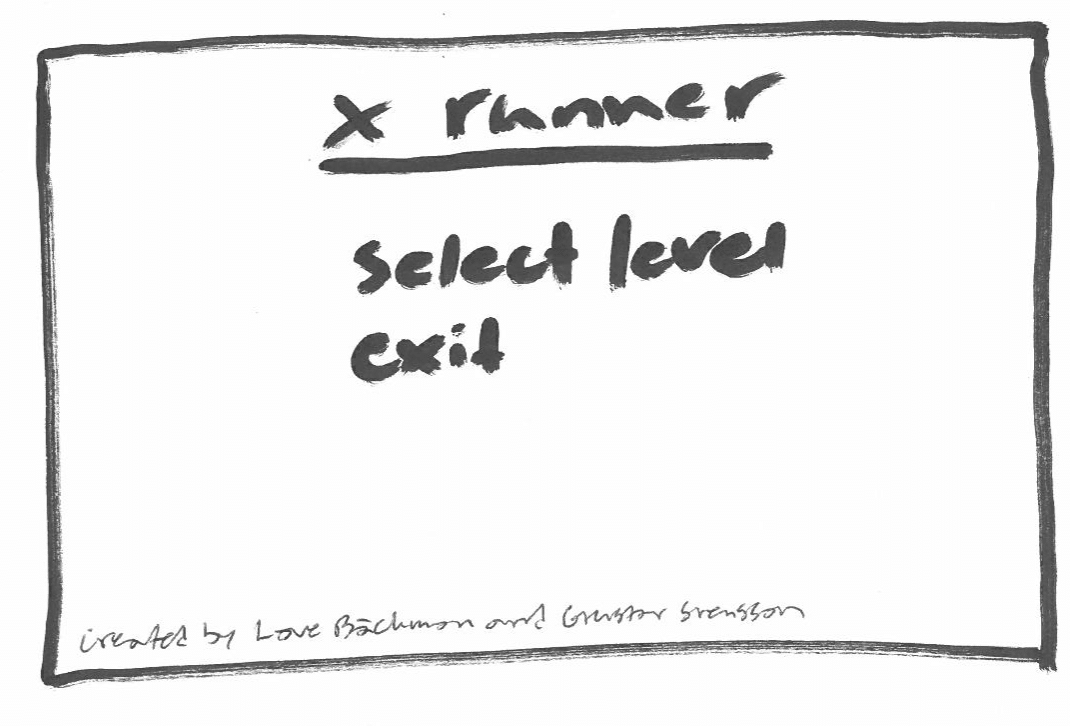
\includegraphics[scale=0.30]{startmeny}
  \caption{Startmenyn}
  \label{Startmenyn}
\end{figure}

\begin{figure}[!h]
  \centering
  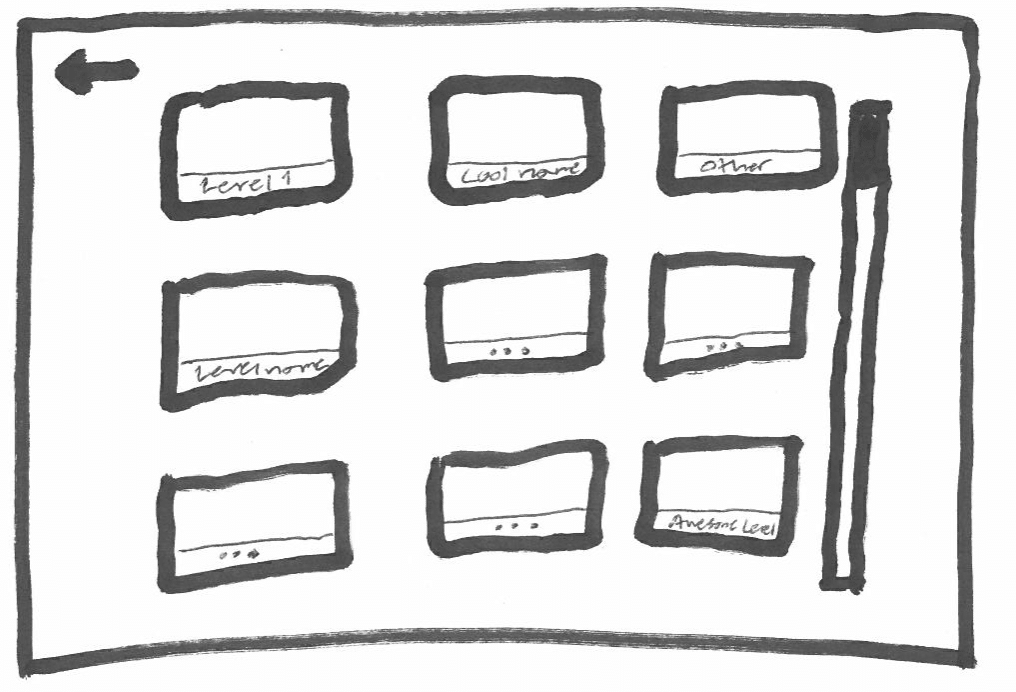
\includegraphics[scale=0.30]{levelmeny}
  \caption{Levelmenyn}
  \label{Levelmenyn}
\end{figure}

\begin{figure}[!h]
  \centering
  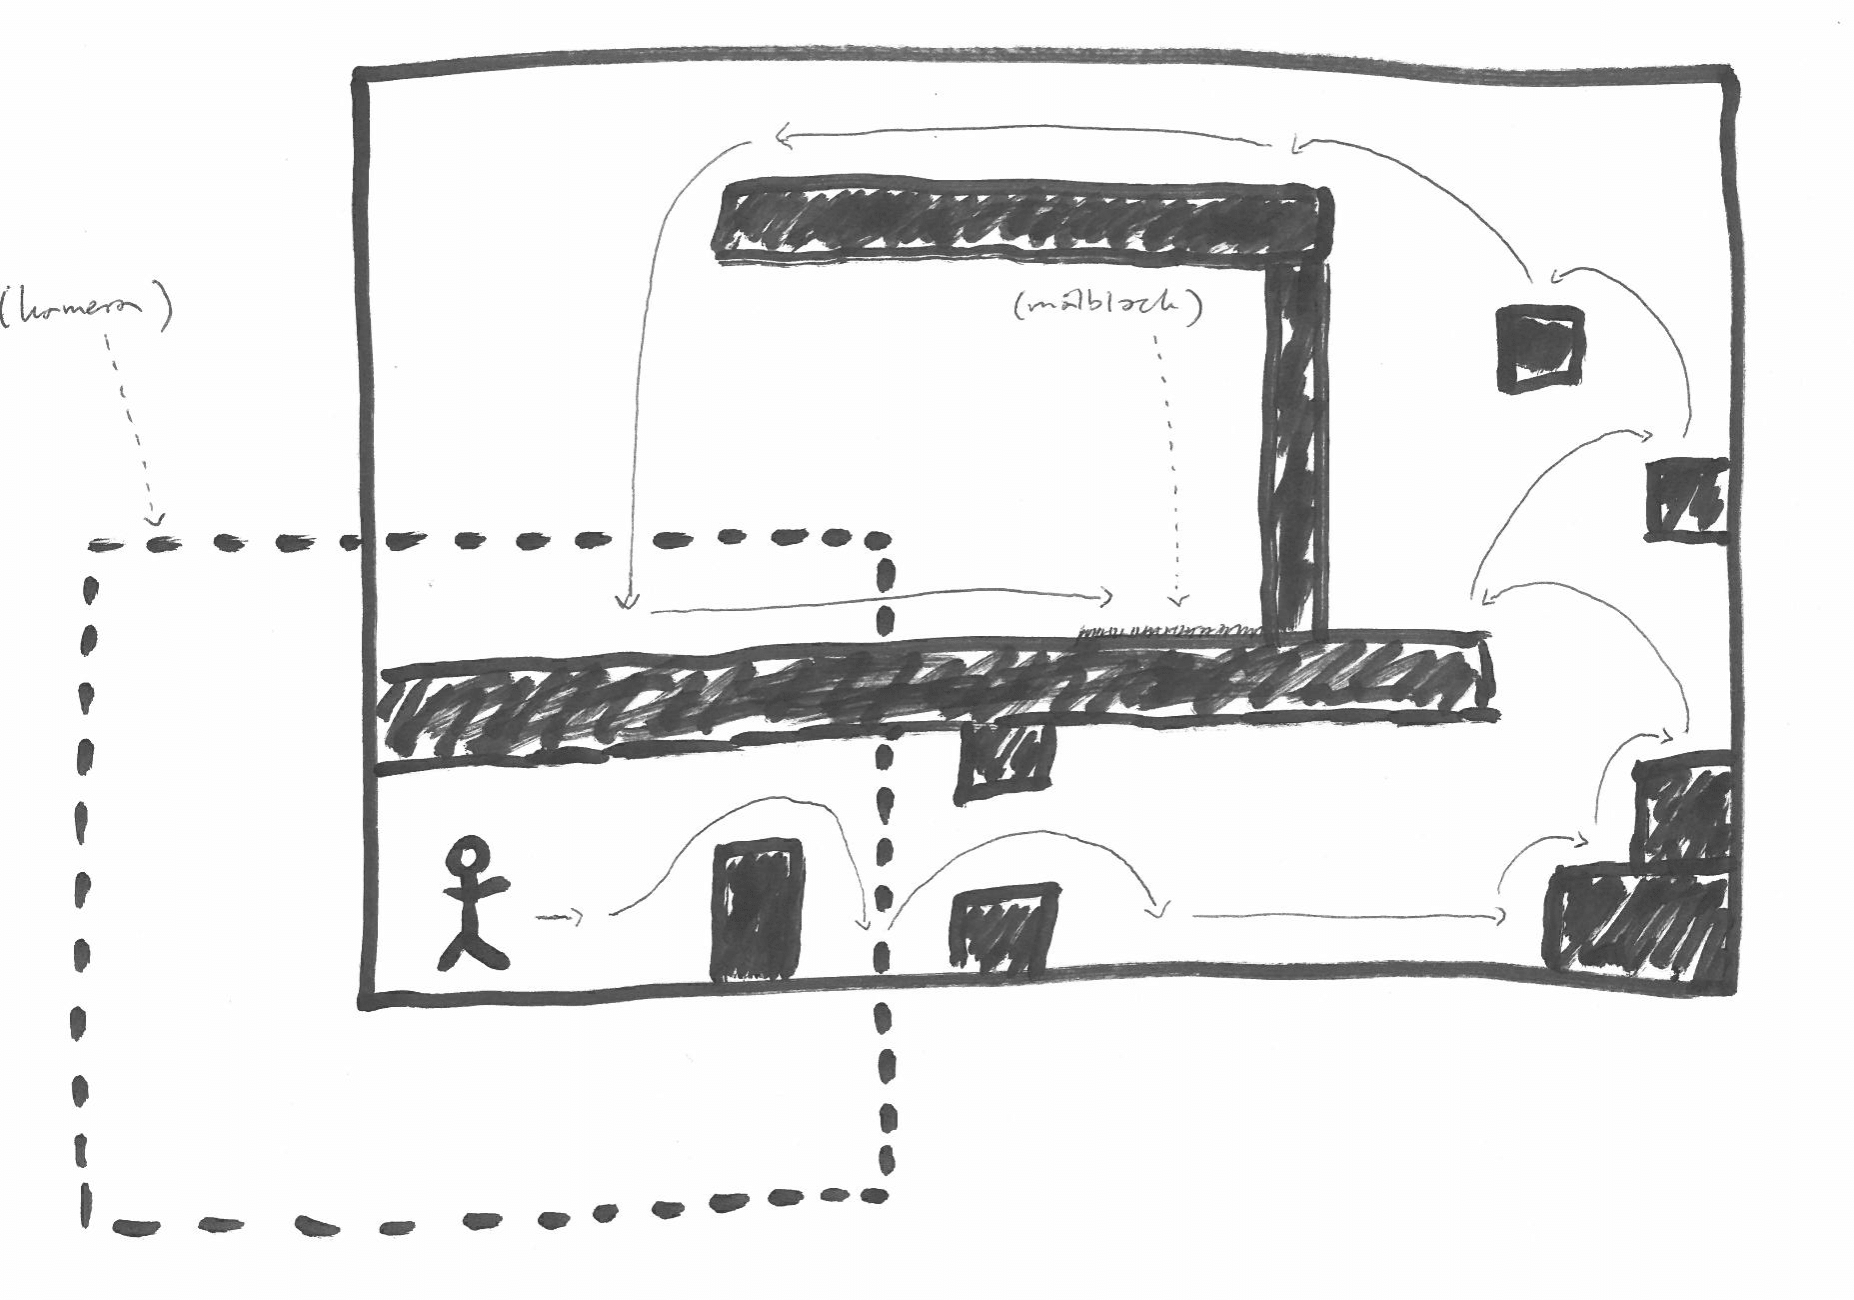
\includegraphics[scale=0.25]{spelplan}
  \caption{Spelplan}
  \label{Spelplan}
\end{figure}

\newpage

\section{Kravformulering}
\subsection{Ska-krav}
\begin{itemize}
\item Spelaren ska kunna flytta sig i sidled och hoppa med tangentbordet.
\item Den valda banan ska kunna målas ut.
\item NPC:er ska kunna röra sig.
\item Det ska kunna finnas flera NPC:er på banan.
\item Inga objekt ( Allting som finns på spelplanen ) ska kunna passera igenom solida block.
\item När spelaren nuddar ett goalblock så ska spelaren ha klarat banan.
\item Spelaren ska alltid vara centrerad på skärmen.
\end{itemize}

\subsection{Bör-krav}
\begin{itemize}
\item Spelet ska spara den bästa tid på varje bana.
\item Man ska kunna spela online multiplayer.
\item Spelarens hastighet ska öka när spelaren hoppar flera gånger i rad utan att kollidera med ett solidt block.
\item Spelaren ska kunna göra ``wall jumps'' genom att hoppa inom en fördefinierad tidsram efter att spelaren har kolliderat med ett solidts blocks vägg.
\item Den bästa för den nuvarande banan ska synas på skärmen.
\item När spelaren nuddar en NPC utförs den ovan definierade händelsen.
\item När spelaren eller NPC:er nuddar ett block så utförs den ovan definierade händelsen.
\item Spelaren ska påverkas av gravitation.
\end{itemize}

\section{Kravuppfyllelse}
\textit{Spelet ska simulera en värld som innehåller olika typer av objekt. Objekten ska ha olika beteenden och röra
sig i världen och agera på olika sätt när de möter andra objekt.}
\begin{itemize}
\item Varje bana har flera olika typer av block och NPC:er som alla har olika beteenden och egenskaper samt interagerar med varandra och spelaren.
\end{itemize}


\noindent\textit{Det måste finnas minst tre olika typer av objekt och det ska finnas flera instanser av minst två av dessa.
T.ex ett spelarobjekt och många instanser av två olika slags fiendeobjekt.}
\begin{itemize}
\item Spelet har flera olika typer av objekt, olika blockobjekt, två olika NPC:er samt spelaren. Det kommer finnas flera olika instancer av dessa.
\end{itemize}

\noindent\textit{Ett beteende som måste finnas med är att figurerna ska röra sig över skärmen. Rörelsen kan följa ett
mönster och/eller vara slumpmässig. Minst ett objekt, utöver spelaren ska ha någon typ av rörelse.}
\begin{itemize}
\item Spelaren ska kunna röra sig i höjdled samt sidled och påverkas av gravitation. NPC:er kommer även kunna röra sig i sidled, eventuellt enligt en sin-/cosinus kurva.
\end{itemize}

\noindent\textit{En figur ska styras av spelaren, antingen med tangentbordet eller med musen. Du kan även göra ett spel där
man spelar två stycken genom att dela på tangentbordet (varje spelare använder olika tangenter). Då styr
man var sin figur.}
\begin{itemize}
\item Spelaren styr sin karaktär genom att använda tangentbordet.
\end{itemize}

\noindent\textit{Grafiken ska vara tvådimensionell.}
\begin{itemize}
\item Ja, vi använder 2D-grafik med hjälp av SFML.
\end{itemize}

\noindent\textit{Världen (spelplanen) kan antas vara lika stor som fönstret (du kan göra en större spelplan med scrollning,
men det blir lite krångligare).}
\begin{itemize}
\item Spelplanen kommer använda scrolling så ja, detta uppfylls.
\end{itemize}

\textit{Det ska finnas kollisionshantering, det vill säga, det ska hända olika saker när objekten möter varandra, 
de ska påverka varandra på något sätt. T.ex kan ett av objekten tas bort, eller så kan objekten förvandlas på
något sätt, eller så kan ett nytt objekt skapas.}
\begin{itemize}
\item Ja, detta uppfylls. När spelaren kolliderar med solida block eller med NPC:er samt när NPC:er kolliderar med solida block.
\end{itemize}

\noindent\textit{Spelet måste upplevas som ett sammanhängande spel som går att spela!}
\begin{itemize}
\item Ja det kommer det att göra.
\end{itemize}

\end{document}
